\chapter{Metodologi dan Desain Sistem}

\section{Perancangan Alur Sistem}

\begin{figure}[H]
\centering

\tikzstyle{startstop} = [
rectangle,
rounded corners,
minimum width=2.8cm,
minimum height=0.8cm,
text centered,
draw=black,
fill=red!20
]

\tikzstyle{process} = [
rectangle,
minimum width=3.5cm,
minimum height=0.8cm,
text centered,
draw=black,
fill=orange!20
]

\tikzstyle{arrow} = [
thick,
->,
>=stealth
]

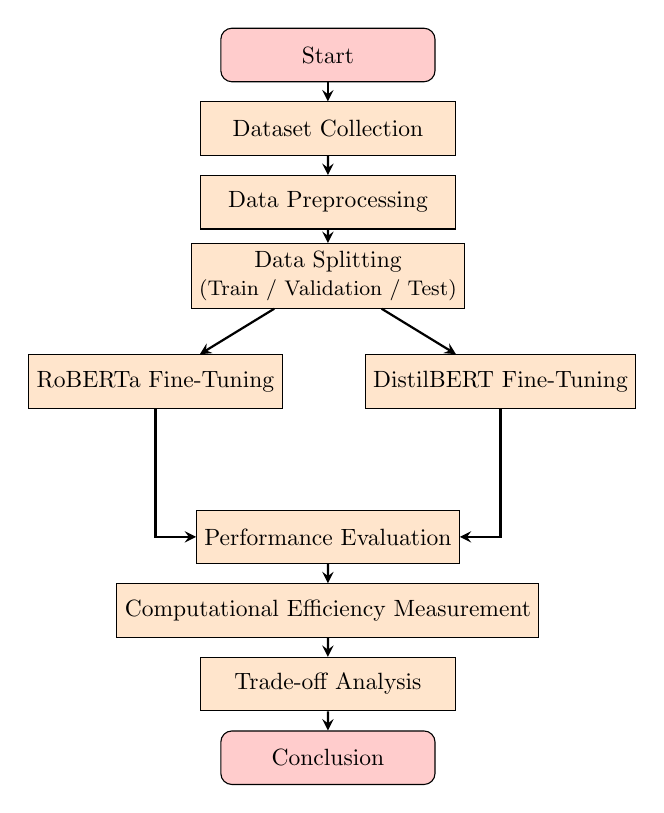
\begin{tikzpicture}[
scale=0.85,
transform shape,
node distance=1.1cm
]

\node (start) [startstop] {Start};

\node (dataset) [process, below of=start]
{Dataset Collection};

\node (preprocess) [process, below of=dataset]
{Data Preprocessing};

\node (split) [process, below of=preprocess]
{\shortstack{Data Splitting\\\small{(Train / Validation / Test)}}};

\node (roberta) [process,
below left of=split,
xshift=-1.8cm,
yshift=-0.8cm]
{RoBERTa Fine-Tuning};

\node (distilbert) [process,
below right of=split,
xshift=1.8cm,
yshift=-0.8cm]
{DistilBERT Fine-Tuning};

\node (evaluation) [process,
below of=split,
yshift=-2.8cm]
{Performance Evaluation};

\node (efficiency) [process, below of=evaluation]
{Computational Efficiency Measurement};

\node (tradeoff) [process, below of=efficiency]
{Trade-off Analysis};

\node (end) [startstop, below of=tradeoff]
{Conclusion};

\draw [arrow] (start) -- (dataset);

\draw [arrow] (dataset) -- (preprocess);

\draw [arrow] (preprocess) -- (split);

\draw [arrow] (split) -- (roberta);

\draw [arrow] (split) -- (distilbert);

\draw [arrow] (roberta) |- (evaluation);

\draw [arrow] (distilbert) |- (evaluation);

\draw [arrow] (evaluation) -- (efficiency);

\draw [arrow] (efficiency) -- (tradeoff);

\draw [arrow] (tradeoff) -- (end);

\end{tikzpicture}

\caption{Research flow of the proposed system}
\label{fig:researchflow}

\end{figure}

Studi ini dilakukan untuk menganalisis \textit{trade-off} antara akurasi klasifikasi dan efisiensi komputasi dalam tugas deteksi sarkasme menggunakan dua model berbasis transformer, yaitu RoBERTa dan DistilBERT. Penelitian ini berfokus pada evaluasi efektivitas kedua model tersebut dalam memahami konteks sarkastis pada teks media sosial. Selain itu, kebutuhan komputasi untuk pelatihan dan inferensi juga dipertimbangkan. Pendekatan ini dipilih karena model arsitektur transformer modern umumnya menunjukkan performa klasifikasi yang tinggi tetapi mahal secara komputasi sehingga kurang cocok untuk implementasi secara \textit{\textit{real-time}} \cite{dubey2025unpacking}.

Alur kerja penelitian umumnya dimulai dengan mengumpulkan dataset sarkasme dari dataset benchmark publik dan media sosial. Data yang terkumpul kemudian diproses melalui serangkaian tahap preprocessing, termasuk penghapusan data \textit{noise}, normalisasi teks, tokenisasi, dan persiapan input agar kompatibel dengan model berbasis transformer. Setelah langkah preprocessing, dataset dibagi menjadi data pelatihan, validasi, dan pengujian. Selanjutnya, pelatihan dilakukan menggunakan skenario yang sama untuk menyempurnakan model RoBERTa dan DistilBERT secara terpisah guna memberikan proses evaluasi yang adil dan konsisten.

Tahap selanjutnya adalah mengevaluasi performa kedua model menggunakan beberapa metrik klasifikasi yang berbeda seperti accuracy, precision, recall, dan F1-score. Studi ini juga mengukur efisiensi komputasi model dalam hal waktu pelatihan, waktu inferensi, penggunaan memori, dan jumlah parameter dalam model. Hasil yang diperoleh dari evaluasi performa dan pengukuran efisiensi komputasi dari kedua model dianalisis untuk melihat hubungan antara kualitas klasifikasi dan kebutuhan sumber daya komputasi untuk setiap model. Gambaran umum tahapan penelitian secara keseluruhan diilustrasikan pada Gambar 3.1. Deskripsi masing-masing tahapan diuraikan pada subbab berikut.

\section{Dataset dan Sumber Data}

Dataset utama yang digunakan dalam penelitian ini adalah \textit{Self-Annotated Reddit Corpus} (SARC). SARC merupakan salah satu dataset \textit{benchmark} yang banyak digunakan dalam deteksi sarkasme karena diekstrak langsung dari forum diskusi Reddit, mencakup komunitas seperti \textit{AskReddit}, \textit{politics}, dan \textit{worldnews}. Dataset ini berisi total sekitar 1,3 juta komentar dengan distribusi kelas yang seimbang, yakni 650.000 komentar sarkastis dan 650.000 komentar non-sarkastis \cite{zhang2025enhancing}.

Karakteristik utama dari dataset SARC adalah struktur percakapannya yang bersifat kontekstual. Ekspresi sarkastis dalam Reddit sering kali implisit dan sangat bergantung pada pemahaman terhadap hubungan \textit{parent-child conversation}, berbeda dengan dataset sentimen tradisional yang umumnya hanya mengevaluasi kalimat tunggal secara terisolasi \cite{dubey2025unpacking}. Kompleksitas kontekstual ini, ditambah dengan tingginya penggunaan ungkapan gaul dan struktur tata bahasa yang tidak konsisten, menjadikannya dataset yang ideal untuk mengevaluasi keandalan model pada wacana media sosial yang realistis.

Pemilihan SARC sebagai dataset utama sesuai dengan tujuan utama penelitian ini, terutama dalam konteks analisis trade-off antara kemampuan klasifikasi dan efisiensi komputasi model berbasis transformer. Struktur percakapan yang panjang dan ketergantungan kontekstual dalam diskusi Reddit memberikan tantangan yang cukup kompleks untuk tugas deteksi sarkasme, di mana hubungan semantik jangka panjang perlu ditangkap secara efektif oleh model. Karakteristik ini membuat SARC sangat sesuai untuk menguji kemampuan pemahaman kontekstual RoBERTa, serta untuk mengevaluasi kemampuan DistilBERT dalam mempertahankan kinerja yang kompetitif dengan kebutuhan komputasi yang lebih rendah \cite{dubey2025unpacking}. Selain itu, ukuran dataset yang besar juga memungkinkan analisis yang lebih komprehensif terhadap waktu pelatihan, kecepatan inferensi, penggunaan memori, dan biaya komputasi secara keseluruhan dalam penerapan model.

Meskipun demikian, dataset SARC memiliki sejumlah tantangan terlepas dari keunggulannya. Dataset ini mengandung ekspresi sarkastis yang sangat ambigu yang mungkin bergantung pada makna implisit, referensi budaya, atau konteks percakapan tertentu. Selain itu, sifat komentar yang \textit{\textit{noise}} di Reddit membuat proses preprocessing dan ekstraksi fitur menjadi lebih sulit. Meskipun demikian, tantangan tersebut menjadi bagian penting dalam penelitian ini karena mampu menyediakan benchmark yang realistis untuk mengevaluasi ketangguhan serta perilaku komputasi model transformer dalam mendeteksi sarkasme pada lingkungan media sosial nyata.

\section{Tahap Preprocessing Data}

Tahap preprocessing data dilakukan untuk mempersiapkan dataset bagi model deteksi sarkasme berbasis transformer. Hal ini sangat penting karena teks media sosial dalam \textit{Self-Annotated Reddit Corpus} (SARC) sangat tidak terstruktur dan penuh dengan \textit{noise}. Komentar pada Reddit umumnya mengandung bahasa informal, singkatan, \textit{slang}, kesalahan penulisan, serta berbagai elemen tambahan seperti URL, \textit{user mentions}, dan emoji. Selain itu, ekspresi sarkastis pada Reddit seringkali bersifat implisit dan sangat bergantung pada konteks percakapan sebelumnya, sehingga preprocessing perlu dilakukan secara hati-hati agar informasi kontekstual dan isyarat sarkasme (\textit{sarcasm cues}) tetap dapat dipertahankan.

Pada penelitian ini, preprocessing dilakukan dalam beberapa langkah utama. Tahap awal meliputi pembersihan teks (text cleaning) dengan menghapus elemen non-semantik seperti URL, tag HTML, komentar duplikat, dan user mentions. Sesuai dengan batasan masalah pada pendekatan unimodal teks, elemen multimodal seperti emoji dihapus agar analisis trade-off komputasi pada arsitektur model dapat diukur secara murni tanpa bias komputasi karakter khusus. Selain itu, teks diseragamkan menjadi huruf kecil (lowercasing) dan tanda baca dihapus untuk mengurangi kompleksitas representasi input sesuai standar pra-pemrosesan model bahasa berbasis transformer. Setelah teks dibersihkan, setiap komentar target akan digabungkan dengan komentar induknya (parent comment) untuk menjaga hubungan konteks pada struktur percakapan Reddit. Pendekatan ini penting karena banyak pernyataan sarkastis tidak dapat diinterpretasikan tanpa mempertimbangkan konteks percakapan sebelumnya\cite{dubey2025unpacking, dubey2026efficient}.

Tahap berikutnya adalah melakukan tokenisasi teks dengan tokenizer bawaan dari setiap arsitektur transformer, yaitu RoBERTaTokenizer dan DistilBertTokenizer. Tokenizer bawaan ini digunakan untuk mempertahankan struktur sintaksis dan representasi kontekstual yang diperlukan oleh model transformer untuk menghasilkan embedding kontekstual. Dengan demikian, teknik \textit{pre-processing} tradisional seperti stemming, \textit{aggressive lemmatization}, dan \textit{stopword removal} tidak dilakukan untuk penelitian ini karena berpotensi menghilangkan hubungan semantik antar kata yang sangat penting untuk deteksi sarkasme. Selain itu, penelitian ini juga menggunakan pengaturan maximum \textit{sequence} length tertentu melalui proses truncation untuk mengontrol panjang input teks agar tetap sesuai dengan kapasitas model dan efisien secara komputasi.

Penerapan preprocessing dalam penelitian ini tidak hanya bertujuan untuk meningkatkan kualitas representasi tekstual, tetapi juga untuk mendukung analisis \textit{trade-off} antara performa model dan efisiensi komputasi. Pengurangan \textit{noise} pada teks memungkinkan mekanisme attention untuk lebih fokus pada isyarat sarkasme yang relevan secara linguistik. Di sisi lain, pengurangan panjang sekuens secara optimal dapat membantu mengurangi waktu pelatihan, penggunaan memori GPU, dan kompleksitas komputasi dalam arsitektur transformer \cite{dubey2025unpacking}. Oleh karena itu, fase preprocessing sangat penting dalam memastikan bahwa evaluasi RoBERTa dan DistilBERT dapat dilakukan secara adil, konsisten, dan sejalan dengan tujuan utama penelitian ini.

\section{Implementasi Model RoBERTa}

\begin{figure}[H]
\centering

% Style definitions
\tikzstyle{startstop} = [rectangle, rounded corners,
minimum width=3.2cm,
minimum height=0.8cm,
text centered,
draw=black,
fill=red!20]

\tikzstyle{process} = [rectangle,
minimum width=3.8cm,
minimum height=0.8cm,
text centered,
draw=black,
fill=orange!20]

\tikzstyle{arrow} = [thick,->,>=stealth]

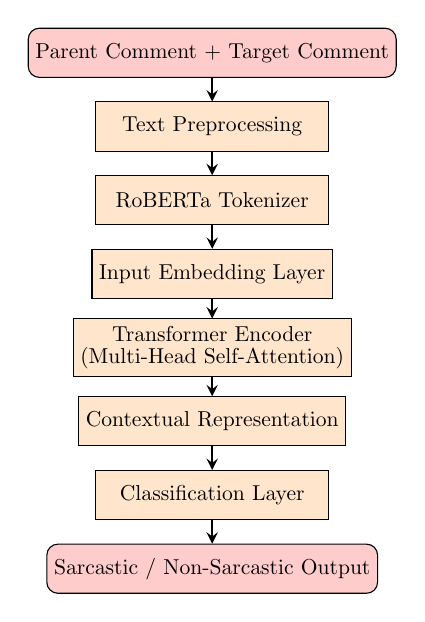
\begin{tikzpicture}[
node distance=1.2cm,
scale=0.78,
transform shape
]

% Nodes
\node (input) [startstop]
{Parent Comment + Target Comment};

\node (preprocess) [process, below of=input]
{Text Preprocessing};

\node (tokenizer) [process, below of=preprocess]
{RoBERTa Tokenizer};

\node (embedding) [process, below of=tokenizer]
{Input Embedding Layer};

\node (encoder) [process, below of=embedding]
{\shortstack{Transformer Encoder \\ (Multi-Head Self-Attention)}};

\node (contextual) [process, below of=encoder]
{Contextual Representation};

\node (classification) [process, below of=contextual]
{Classification Layer};

\node (output) [startstop, below of=classification]
{Sarcastic / Non-Sarcastic Output};

% Arrows
\draw [arrow] (input) -- (preprocess);
\draw [arrow] (preprocess) -- (tokenizer);
\draw [arrow] (tokenizer) -- (embedding);
\draw [arrow] (embedding) -- (encoder);
\draw [arrow] (encoder) -- (contextual);
\draw [arrow] (contextual) -- (classification);
\draw [arrow] (classification) -- (output);

\end{tikzpicture}

\caption{Architecture of RoBERTa implementation for sarcasm detection on the SARC dataset}
\label{fig:robertaflow}

\end{figure}

Pada penelitian ini, RoBERTa digunakan sebagai salah satu model berbasis transformer utama untuk deteksi sarkasme pada dataset \textit{Self-Annotated Reddit Corpus} (SARC). RoBERTa \textit{(Robustly Optimized BERT Pretraining Approach)} adalah versi modifikasi dari arsitektur BERT yang dioptimalkan untuk pemahaman konteks bahasa yang lebih baik melalui \textit{pre-training} yang lebih optimal. RoBERTa memperkenalkan beberapa peningkatan arsitektural dibandingkan model BERT standar, termasuk \textit{dynamic masking}, penghapusan objektif \textit{Next Sentence Prediction} (NSP), dan pelatihan dataset yang lebih besar untuk jangka waktu yang lebih lama. Peningkatan tersebut memungkinkan RoBERTa menghasilkan representasi kontekstual yang lebih kaya dan mampu menangkap hubungan semantik antar kata dengan lebih baik.

Penelitian ini menggunakan model RoBERTa karena sifat sarkasme yang bergantung pada konteks dalam percakapan media sosial. Ucapan sarkastis biasanya dipahami sebagai kebalikan dari apa yang diucapkan secara harfiah dan seringkali memerlukan konteks percakapan sebelumnya agar dapat diinterpretasikan dengan benar. Model RoBERTa menggunakan mekanisme \textit{multi-head self-attention} yang memungkinkan model untuk menganalisis hubungan antar kata dan petunjuk konteks secara bersamaan, sehingga sangat sesuai untuk mengidentifikasi sarkasme implisit pada diskusi Reddit. Selain itu, kemampuan \textit{contextual embedding} RoBERTa memungkinkan model untuk menangani teks media sosial yang \textit{noise} dan informal dengan lebih baik, seperti bahasa gaul, singkatan, dan struktur tata bahasa yang tidak konsisten, yang sering ditemukan dalam dataset SARC \cite{dubey2025unpacking, jimenez2026bert}.

Proses implementasi dimulai dengan menggunakan RoBERTaTokenizer untuk melakukan tokenisasi teks hasil preprocessing sebelumnya. Setiap input terdiri dari komentar target yang digabungkan dengan \textit{parent comment} untuk mempertahankan konteks percakapan dalam struktur diskusi Reddit. Hasil tokenisasi kemudian dikonversi menjadi \textit{contextual embedding} melalui beberapa lapisan encoder transformer. Pada tahap fine-tuning, model RoBERTa yang telah dilatih sebelumnya disesuaikan dengan tugas deteksi sarkasme dengan data berlabel dari dataset SARC. Representasi kontekstual terakhir dari encoder transformer dilewatkan melalui lapisan klasifikasi dengan fungsi aktivasi Softmax untuk memprediksi kelas komentar (sarkastis atau non-sarkastis).

Meskipun RoBERTa memiliki pemahaman kontekstual yang sangat baik, arsitektur ini menghadirkan tantangan biaya komputasi yang substansial. Secara bawaan, mekanisme \textit{self-attention} pada \textit{transformer} memiliki tingkat kompleksitas yang tinggi, yang menjadi semakin membebani ketika memproses sekuens teks panjang dari kumpulan data berskala besar seperti SARC. Akibatnya, RoBERTa menuntut kapasitas memori GPU yang masif, waktu pelatihan yang lebih lambat, serta menghasilkan latensi inferensi yang jauh lebih tinggi dibandingkan model \textit{transformer} ringan (\textit{lightweight}) \cite{dubey2025unpacking}. Namun demikian, karakteristik komputasi yang berat inilah yang justru menjadikan RoBERTa sangat relevan dengan tujuan penelitian ini, yaitu sebagai representasi model berkinerja tinggi untuk menganalisis \textit{trade-off} antara akurasi klasifikasi dan efisiensi komputasi pada sistem deteksi sarkasme.

\section{Implementasi Model DistilBERT}

\begin{figure}[H]
\centering

% Style definitions
\tikzstyle{startstop} = [rectangle, rounded corners,
minimum width=3.2cm,
minimum height=0.8cm,
text centered,
draw=black,
fill=red!20]

\tikzstyle{process} = [rectangle,
minimum width=3.8cm,
minimum height=0.8cm,
text centered,
draw=black,
fill=orange!20]

\tikzstyle{arrow} = [thick,->,>=stealth]

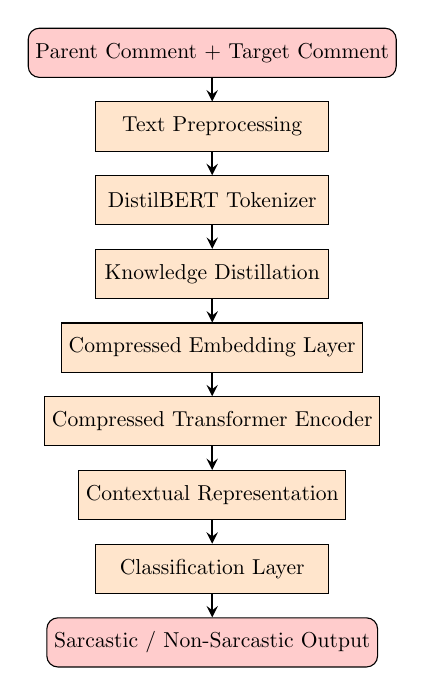
\begin{tikzpicture}[
node distance=1.2cm,
scale=0.78,
transform shape
]

% Nodes
\node (input) [startstop]
{Parent Comment + Target Comment};

\node (preprocess) [process, below of=input]
{Text Preprocessing};

\node (tokenizer) [process, below of=preprocess]
{DistilBERT Tokenizer};

\node (distillation) [process, below of=tokenizer]
{Knowledge Distillation};

\node (embedding) [process, below of=distillation]
{Compressed Embedding Layer};

\node (encoder) [process, below of=embedding]
{Compressed Transformer Encoder};

\node (contextual) [process, below of=encoder]
{Contextual Representation};

\node (classification) [process, below of=contextual]
{Classification Layer};

\node (output) [startstop, below of=classification]
{Sarcastic / Non-Sarcastic Output};

% Arrows
\draw [arrow] (input) -- (preprocess);
\draw [arrow] (preprocess) -- (tokenizer);
\draw [arrow] (tokenizer) -- (distillation);
\draw [arrow] (distillation) -- (embedding);
\draw [arrow] (embedding) -- (encoder);
\draw [arrow] (encoder) -- (contextual);
\draw [arrow] (contextual) -- (classification);
\draw [arrow] (classification) -- (output);

\end{tikzpicture}

\caption{Architecture of DistilBERT implementation for sarcasm detection on the SARC dataset}
\label{fig:distilbertflow}

\end{figure}

Pada penelitian ini, kami menggunakan DistilBERT sebagai model pembanding berbasis transformer untuk menganalisis trade-off antara performa klasifikasi dan efisiensi komputasi dalam tugas pendeteksian sarkasme. DistilBERT merupakan versi ringan (lightweight transformer) dari arsitektur BERT yang dikembangkan menggunakan teknik knowledge distillation. Pendekatan ini memungkinkan model untuk mewarisi pengetahuan dari arsitektur transformer yang lebih besar, sambil mempertahankan sebagian besar kemampuannya untuk memahami konteks. DistilBERT mengurangi sekitar 40\% lapisan yang digunakan dalam arsitektur BERT standar. Hal ini menghasilkan ukuran parameter yang lebih kecil dan kompleksitas komputasi yang lebih rendah.

Penggunaan DistilBERT didasarkan pada kebutuhan sistem deteksi sarkasme yang tidak hanya kompetitif secara performa, tetapi juga adaptif secara operasional. Pada platform media sosial seperti Reddit, sistem berpotensi diterapkan pada skenario \textit{real-time} dengan volume data masif yang menuntut latensi inferensi sangat rendah. Sebagai alternatif dari model berat seperti RoBERTa, DistilBERT menawarkan kecepatan pelatihan dan inferensi yang jauh lebih tinggi. Meskipun mengalami kompresi arsitektural yang signifikan, DistilBERT terbukti secara empiris mampu mempertahankan kapasitas pemahaman kontekstual yang memadai untuk menangkap ekspresi sarkasme yang implisit di dalam wacana sosial \cite{dubey2025unpacking}.

Proses implementasi dimulai dengan tahap tokenisasi teks yang sudah diproses sebelumnya menggunakan DistilBertTokenizer. Setiap input terdiri dari komentar target yang digabungkan dengan komentar induknya (parent comment) untuk mempertahankan konteks percakapan Reddit, seperti pada implementasi RoBERTa. Hasil tokenisasi kemudian diubah representasi contextual embeddings melalui beberapa lapisan transformer encoder yang terkompresi. Pada tahap fine-tuning, model DistilBERT disesuaikan dengan tugas klasifikasi sarkasme menggunakan dataset SARC yang telah diberi label. Representasi kontekstual terakhir kemudian diteruskan melalui lapisan klasifikasi dengan fungsi aktivasi Softmax untuk memprediksi kelas sarkastis dan non-sarkastis.

Keuntungan utama dari DistilBERT adalah efisiensi komputasinya. Parameter yang lebih sedikit memungkinkan model ini menggunakan memori GPU yang jauh lebih rendah, mempercepat waktu pelatihan, dan memangkas latensi inferensi dibandingkan dengan RoBERTa. Karakteristik ini membuat DistilBERT sangat ideal untuk diterapkan di lingkungan dengan keterbatasan sumber daya maupun kebutuhan pemrosesan \textit{real-time}. Meskipun demikian, arsitektur DistilBERT yang dikompresi juga berdampak pada berkurangnya kedalaman representasi kontekstual. Hal ini menyebabkan performa klasifikasinya sedikit lebih rendah dibandingkan RoBERTa, terutama ketika berhadapan dengan kasus sarkasme yang sangat implisit dan kompleks \cite{dubey2025unpacking}. Oleh karena itu, penerapan DistilBERT dalam penelitian ini menjadi krusial untuk mengevaluasi sejauh mana efisiensi komputasi dapat dicapai tanpa menimbulkan degradasi yang signifikan pada performa deteksi sarkasme..

\section{Metode Evaluasi dan Pengukuran Kinerja}

Dalam penelitian ini, model RoBERTa dan DistilBERT untuk deteksi sarkasme dievaluasi dalam hal kinerja klasifikasi dan efisiensi komputasi menggunakan dataset SARC. Proses evaluasi tidak hanya mempertimbangkan kemampuan model dalam mengklasifikasikan komentar sarkastis dan non-sarkastis secara akurat, tetapi juga sumber daya komputasi yang diperlukan untuk pelatihan dan inferensi. Sebagai hasilnya, penelitian ini menggunakan dua kategori utama evaluasi, yaitu metrik kinerja klasifikasi dan metrik efisiensi komputasi.

\subsection{Classification Performance Metrics}

Evaluasi performa klasifikasi dilakukan untuk mengetahui kemampuan model RoBERTa dan DistilBERT dalam membedakan komentar sarkastis dan non-sarkastis pada dataset pengujian. Untuk memperoleh gambaran performa yang lebih menyeluruh, penelitian ini menggunakan metrik \textit{accuracy}, \textit{precision}, \textit{recall}, dan \textit{F1-score}.

Masing-masing metrik memberikan sudut pandang yang berbeda dalam proses evaluasi. \textit{Accuracy} digunakan untuk melihat tingkat ketepatan prediksi model secara keseluruhan, sedangkan \textit{precision} dan \textit{recall} digunakan untuk menilai kemampuan model dalam mengidentifikasi komentar yang mengandung sarkasme. Selain itu, \textit{F1-score} digunakan sebagai metrik utama karena mampu merepresentasikan keseimbangan antara \textit{precision} dan \textit{recall}, sehingga dapat memberikan gambaran yang lebih objektif terhadap performa model.

Perhitungan dan definisi masing-masing metrik mengacu pada landasan teori yang telah dijelaskan pada Subbab 2.3.

\subsection{Computational Efficiency Metrics}

Selain mengevaluasi performa klasifikasi, penelitian ini juga menilai efisiensi komputasi dari setiap model yang digunakan. Evaluasi tersebut dilakukan untuk mengetahui besarnya sumber daya komputasi yang dibutuhkan selama proses pelatihan maupun inferensi, sehingga dapat memberikan gambaran mengenai kelayakan penerapan model pada kondisi nyata.

Pengukuran efisiensi komputasi dilakukan menggunakan beberapa metrik, yaitu \textit{training time}, \textit{inference latency}, penggunaan memori GPU, dan jumlah parameter model. \textit{Training time} digunakan untuk mengukur waktu yang diperlukan selama proses \textit{fine-tuning}, sedangkan \textit{inference latency} digunakan untuk melihat kecepatan model dalam menghasilkan prediksi pada data pengujian. Penggunaan memori GPU diamati untuk mengetahui kebutuhan sumber daya selama proses pelatihan, sementara jumlah parameter model digunakan sebagai indikator kompleksitas arsitektur yang dimiliki oleh masing-masing model.

Definisi dan dasar teori dari metrik efisiensi komputasi yang digunakan dalam penelitian ini mengacu pada Subbab 2.3.

\subsection{Trade-off Analysis}

Tahap evaluasi akhir dilakukan melalui analisis trade-off antara performa klasifikasi dan efisiensi komputasi dari RoBERTa dan DistilBERT. Analisis ini tidak bertujuan untuk menentukan satu model yang terbaik secara mutlak, tetapi untuk melihat seberapa besar perubahan performa yang terjadi dibandingkan dengan keuntungan efisiensi komputasi yang diperoleh.

Performa klasifikasi dibandingkan berdasarkan accuracy, precision, recall, dan F1-score, sedangkan efisiensi komputasi dibandingkan berdasarkan training time, inference latency, penggunaan memori GPU, dan jumlah parameter model. Perbedaan tersebut kemudian dianalisis dalam bentuk penurunan performa (performance loss) dan peningkatan efisiensi (efficiency gain), termasuk speedup factor untuk melihat perbedaan kecepatan antara kedua model.

Hasil analisis digunakan untuk melihat kondisi penggunaan masing-masing model. RoBERTa dapat lebih sesuai ketika performa klasifikasi menjadi prioritas, sedangkan DistilBERT dapat lebih sesuai ketika efisiensi komputasi dan keterbatasan sumber daya menjadi pertimbangan utama.


\section{Skenario Pengujian dan Analisis Trade-off}

Dalam penelitian ini, skenario pengujian dirancang untuk membandingkan performa klasifikasi dan efisiensi komputasi RoBERTa dan DistilBERT pada dataset SARC. Agar perbandingan dilakukan secara adil, kedua model menggunakan dataset, preprocessing, struktur input parent comment dan target comment, serta lingkungan komputasi yang sama.

Dataset yang digunakan berupa sekitar 200.000 pasangan parent comment–target comment yang dipilih secara terkontrol dari SARC. Data kemudian dibagi secara stratified menjadi 80\% data pelatihan, 10\% data validasi, dan 10\% data pengujian. Panjang maksimum input ditetapkan sebesar 256 token. Sebelum eksperimen utama dilakukan, pengujian awal menggunakan sekitar 20.000–50.000 data dilakukan untuk memastikan pipeline berjalan dengan baik serta menentukan batch size yang sesuai dengan kapasitas GPU.

Eksperimen utama dilakukan menggunakan GPU NVIDIA RTX 5070 Ti dengan VRAM 16 GB yang tersedia di AI Lab. Proses pelatihan menggunakan mixed precision atau FP16 untuk menyesuaikan kebutuhan komputasi dengan kapasitas perangkat keras. Google Colab dan perangkat pribadi hanya digunakan untuk tahap pengembangan, preprocessing, serta pengujian awal, sedangkan seluruh pengukuran akhir dilakukan pada perangkat GPU yang sama agar hasil perbandingan tetap konsisten.

Setiap model dilatih sebanyak tiga kali menggunakan random seed yang sama untuk mengurangi kemungkinan hasil dipengaruhi oleh satu kali proses pelatihan. Konfigurasi fine-tuning seperti learning rate, batch size, dan jumlah epoch dapat disesuaikan dengan karakteristik masing-masing model, tetapi proses penentuannya dilakukan dengan prosedur yang sama agar perbandingan tetap adil.

Performa klasifikasi dievaluasi menggunakan accuracy, precision, recall, dan F1-score. Efisiensi komputasi diukur berdasarkan training time, inference latency, penggunaan memori GPU, dan jumlah parameter model. Hasil dari ketiga pengujian kemudian dirangkum untuk melihat konsistensi performa dan kebutuhan komputasi masing-masing model.

Analisis trade-off dilakukan dengan membandingkan perubahan performa klasifikasi terhadap keuntungan efisiensi komputasi yang diperoleh. Selain itu, perbedaan kecepatan antara kedua model dihitung menggunakan speedup factor \cite{dubey2025unpacking}:

\[
\text{Speedup Factor} =
\frac{T_{\text{RoBERTa}}}{T_{\text{DistilBERT}}}
\]

Pengukuran tersebut dilakukan secara terpisah untuk waktu pelatihan dan latensi inferensi. Hasil akhir digunakan untuk melihat kondisi penggunaan masing-masing model, yaitu ketika performa klasifikasi menjadi prioritas utama, ketika keterbatasan sumber daya menjadi pertimbangan utama, maupun ketika diperlukan keseimbangan antara keduanya.

